\documentclass[10pt,a4paper]{article}
\usepackage[T1]{fontenc}
\usepackage[brazil]{babel}
\usepackage[utf8]{inputenc}


\usepackage{ae,aecompl}
\usepackage{pslatex}
\usepackage{epsfig}
\usepackage{geometry}
\usepackage{url}
\usepackage{textcomp}
\usepackage{ae}
\usepackage{subfig}
\usepackage{indentfirst}
\usepackage{textcomp}
\usepackage{color}
\usepackage{setspace}
\usepackage{verbatim}
\usepackage{amsmath}
\include{abaco} 


\onehalfspacing
\begin{document}

% CAPA
\thispagestyle{empty}

\begin{minipage}[h]{0.10\linewidth}
  \ABACO{1}{9}{6}{9}{0.5} 
\end{minipage}
\begin{minipage}[h!]{0.7\linewidth}
  \vspace*{\fill}
  \centering
  {\large \textbf{UNIVERSIDADE~ESTADUAL~DE~CAMPINAS}}\\ 
  {\large INSTITUTO~DE~COMPUTAÇÃO}                   
  \vspace*{\fill} 
\end{minipage}
\\\vspace{0.5cm}

\begin{center} 
  \rule{11.0cm}{0.4pt}\vspace*{-\baselineskip}\vspace{-2.0pt}
  \rule{11.0cm}{1.6pt} \vspace*{-\baselineskip}
  {\Large \textsc{Reconhecimento de faces em redes sociais}}\vspace{3.2pt}
  \rule{11.0cm}{0.4pt}\vspace*{-\baselineskip}\vspace{3.2pt} \rule{11.0cm}{1.6pt}\\
  {\textsl{Proposta de projeto}}
  \\\vspace{1cm}
  \begin{tabular}{ll}
    Carlos Eduardo Rosa Machado & \textbf{RA}: 059582\\
    \multicolumn{2}{c}{\small \emph ra059582@students.ic.unicamp.br}  \\
    Douglas Alves Germano        & \textbf{RA}: 060210\\
    \multicolumn{2}{c}{\small \emph ra060210@students.ic.unicamp.br } \\
    Tiago Chedraoui Silva        & \textbf{RA}: 082941\\
    \multicolumn{2}{c}{\small \emph ra082941@students.ic.unicamp.br} \\
  \end{tabular}
\end{center}
\vspace{0.5cm}
\begin{abstract}


  O Facebook é uma rede social , e atualmente possui mais de 700 milhões
  de usuários. Muitas vezes, encontrar um usuário  a partir de
  informações não é algo fácil.
  
  De forma a fornecer mais um método para encontrar um usuário,
  criou-se um sistema que, dado uma foto de entrada contendo uma face
  a ser procurada,  retorna os perfis no Facebook com os rostos mais
  semelhantes ao objetivo dentre os amigos de amigos do usuário.
  
  Não obstante as dificuldade de se comparar faces, através da
  utilização do PCA conseguiu-se para faces retiradas de fotos
  diferentes dos perfis de cada 80 fotos encontrar 50, por outro
  lado,se a imagem fornecida é a mesma do perfil há um grande
  valor de acerto.
\end{abstract}

\tableofcontents
\newpage 
\doublespacing

\section{Introdução e Motivação}
Rede social é uma estrutura composta por indivíduos ou organizações, chamados de nós, que se conectam por um ou vários tipos de relações, tais como amizade, parentesco, interesses em comum, entre outras.

O Facebook é uma rede social gratuita, fundada em 2004, e atualmente possui mais de 700 milhões de usuários ativos.

Uma pessoa pode criar um perfil na rede social, tornando-se um usuário do sistema. Para a criação de um perfil, ela deve fornecer informações pessoais como nome, localização, endereço eletrônico, e outras que desejar. Entre as opções, o usuário pode fornecer uma foto para ser mostrada no perfil, que qualquer outro usuário terá acesso irrestrito e a possibilidade de visualizá-la. Ainda assim, esta é uma prática bastante utilizada pela maioria dos usuários, pois proporciona fácil reconhecimento pelas demais pessoas. Além disso, o usuário pode colocar outras fotos pessoais, para as quais controlará o acesso, deixando restrito, por exemplo, apenas para aqueles que fazem parte da sua rede de relacionamentos no sistema.

Pelo próprio intuito da rede, um usuário cadastrado quer se conectar e se relacionar virtualmente com as pessoas que conhece, ou até mesmo conhecer pessoas novas, quando algum interesse mútuo ocorre.

Desta forma, o Facebook tem algumas ferramentas à disposição dos usuários, que permitem pessoas serem encontradas por outras usando alguma informação, tal como nome, endereço eletrônico ou endereço físico.

Por isso, a ambição do projeto está em criar uma nova ferramenta, um novo meio para que as pessoas se encontrem e se conheçam. Apesar do Facebook ter bons buscadores que encontram facilmente uma pessoa, precisamos sempre ter alguma informação da pessoa, que podemos não saber e não conseguir obter rapidamente. Contudo, podemos ter uma foto, e é neste caso que entra a nossa proposta de solução: buscar um perfil dado uma foto.
\newpage
\section{O problema}
Participar ativamente de uma rede social, tal qual o Facebook, está muito ligado em encontrar seus amigos online e fazer novos amigos, para assim trocar mensagens com os usuários, participar de eventos, estar presente em grupos, entre outras possibilidades. Por conseguinte, o problema consiste em conectar estes usuários, de modo que amigos recentes ou velhos amigos possam ser encontrados facilmente.

É esperado que uma pessoa saiba, ou tenha anotado em algum lugar, informações básicas sobre seus amigos. Porém, nem sempre nos recordamos ou temos estes dados em mãos. Por exemplo, você acabou de conhecer uma pessoa, que por falta de tempo ou por distração, não perguntou o nome dela. Mas, como estavam numa festa e você tirou diversas fotos, acabou reconhecendo ela em uma das diversas fotos que nem se lembra de ter tirado. Assim, com as atuais ferramentas que o Facebook disponibiliza, você não seria capaz de encontrá-la facilmente, pois não sabe nada sobre a pessoa.

A proposta deste projeto é incluir uma ferramenta diferente, que não precisa de qualquer tipo de informação sobre o indivíduo, mas que seja capaz de encontrá-lo por comparação da imagem alvo, esta que você possui na sua câmera, com as imagens dos perfis dos usuários.

Ou seja, o usuário fornece a foto com o rosto da pessoa que deseja buscar, o sistema (e eventualmente um aplicativo) varre a rede procurando as imagens mais semelhantes e retorna os perfis que contêm os rostos mais parecidos, e eventualmente, o perfil correto do usuário buscado.

De início, surgem dois problemas: encontrar uma face dado uma imagem e encontrar esta face em outras imagens. Dado que temos isto, uma ferramenta capaz de reconhecer as características de um ser humano e recortar seu rosto, e outra que faça a comparação das faces detectadas, surge um problema bônus: a imensa quantidade de usuários cadastrados no Facebook.

São centenas de milhões de pessoas ativas especificamente no Facebook, e portanto, fazer a comparação entre todos estes usuários em tempo razoável é uma outra dificuldade a ser enfrentada.

Deste modo, este projeto se propõe a fornecer um novo meio de encontrar usuários na rede utilizando apenas uma foto, mas que dê algum resultado, seja ele de sucesso ou fracasso, em um tempo hábil, mantendo a satisfação do cliente.

Existem outros problemas com os quais lidaremos, mas que não temos muito o que fazer para saná-los, tais como: perfil criado sem foto ou que a foto não seja da pessoa, imagens ruins, ou então que não contenha um rosto.

\section{Solução proposta}
A abordagem tomada foi de criar um aplicativo externo ao Facebook, que utiliza das formas de conexões desenvolvidas e publicadas pela empresa, para interagir e manipular os dados necessários ao nosso projeto.

\subsection*{Definição do espaço:}

A primeira precaução do grupo foi definir o espaço de busca do algoritmo. Dado que o Facebook registra em torno de 700 milhões de usuários ativos no sistema, fazer a comparação entre todos e retornar um resposta adequada seria improvável, pois algoritmos semelhantes, como o do Picasa, demora 6 dias para comprar 50 mil fotos, tempo totalmente fora do esperado pelo usuário.

Portanto, partimos da premissa que a pessoa buscada talvez seja um amigo de um amigo do usuário e limitamos nesta fronteira. Se um usuário médio tem em torno de 130 amigos na rede, estaríamos nos propondo a realizar a busca por 16900 usuários (130 x 130) no caso médio. Esta abordagem nos pareceu bastante favorável, para um retorno satisfatório num tempo adequado.

\subsection*{Graph API:}

O Facebook disponibiliza uma plataforma de desenvolvimento para qualquer pessoa que esteja interessado em iniciar um programa e utilizar das informações contidas nos perfis dos usuários. Vale ressaltar que nem todos os dados pessoais são públicos, a menos que o usuário habilite para que sejam. Entretanto, ao menos a foto do seu perfil, ponto de interesse do projeto, será visualizável a qualquer um.

Toda informação está no que eles chamam de grafo social, onde qualquer coisa é um nó, com identificador único, e possue relações com outros nós. Por exemplo, um usuário X é um nó e está conectado com outro usuário Y, também nó, por uma relação de amizade. São nós: usuários, eventos, fotos, páginas e etc. E são conexões: amizade, participação em eventos, marcação em fotos e outros.

Tudo isto está disposto numa arquitetura de JSON facilmente entendida. Um JSON é composto por uma propriedade e seu valor. Ou seja, para um usuário teremos, por exemplo, a propriedade nome e o seu valor, seu nome.

\subsection*{Python:}

Com as informações obtidas do Graph API, e conhecendo sua estrutura formada por JSON, optamos por utilizar python para desenvolvimento. Se mostrou interessante num primeiro momento, pela grande facilidade de realizar conexões com o Facebook e de manipular as respostas recebidas em formato JSON.

Porém, por ser uma linguagem interpretada, ganhamos em simplicidade e perdemos em processamento, pois uma linguagem compilada seria mais veloz.


\subsection*{PCA:}

O PCA (Principal component analysis) busca um modelo computacional que
melhor descreve uma face extraindo as informações mais relevantes de
uma face. A abordagem de autofaces é um método PCA, em que um pequeno
conjunto de figuras características são usadas para descrever a
variação entre as imagens de faces.

O objetivo é encontrar autovetores(autofaces) da matriz de covariância
da distribuição, calibrado através de treino que utiliza um conjunto
de imagens de faces. Posteriormente, toda imagem é representada pela
combinação linear desses autovetores.

O reconhecimento é realizado através da projeção de uma nova imagem no
subespaço calibrado pelas autofaces e, então, calssifica-se a face
comparando a posição da face no espaço com a posição das faces conhecidas.
Abaixo segue a explicação mais detalhada do processo:

\subsubsection*{Treinamento:}

Sejam $\Gamma_1, \Gamma_2, \Gamma_3, \ldots, \Gamma_m$ as imagens de
faces para treinamento. A face média é definida por {$\Psi
  =\frac{1}{M}* \sum_{i=1}^m\Gamma_i$}. Cada face difere da média pelo vetor {$\Phi_i = \Gamma_i - \Psi$}.

Queremos, através do PCA, obter M vetores ortonormais, $u_n$, que
melhor descrevem a distribuição dos dados. O k-ésimo vetor é escolhido
de tal  forma que


\begin{equation}
  \lambda_{k}=\frac{1}{M}\sum_{n=1}^{M}(u_k^T\Phi_n)^2
\end{equation}

é um máximo, sujeito a

\begin{equation}
  u_l^Tu_k=\delta_{lk}=\left \{
    \begin{array}{l l}
      1, & \quad \text{se $l=k$} \\
      0, & \quad \text{caso contrário}\\
    \end{array}
  \right.
\end{equation}

Os vetores $u_k$ e escalares $\lambda_k$ são os autovalores e autovetores da matriz de covariância

\begin{equation}
  C=\frac{1}{M}\sum_{n=1}^{M}(\Phi_n\Phi_n^T)= AA^T
\end{equation}

onde $A = [ \Phi_1 \Phi_2 \ldots \Phi_m ]$, matriz na qual cada coluna
é uma das faces de treinamento. Supondo que cada imagem de face é
composta por N pixels, esta matriz C será, então, $N^2 x
N^2$. Todavia, se o número de rostos for bem menor do que o tamanho de
cada foto ($M << N$), podemos simplificar os cálculos, se
considerarmos a matriz $A^T * A$ (A transposta vezes A):

\begin{equation}
  A^TAv_i=\mu_iv_i
\end{equation}


Nesse caso, $\mu_i$ e $v_i$ são, respectivamente, os autovalores e
autovetores de $A^T * A$. Multiplicando ambos os lados por A, temos:

\begin{equation}
  AA^TAv_i=\mu_iAv_i
\end{equation}


De onde vemos que $A*v_i$ são os autovetores da matriz original $C = A.A^T$.

Se, por exemplo, temos 300 imagens, cada uma com 100 x 100 pixels,
teremos, então, que resolver uma matriz de $9*10^4$ elementos, ao
invés de $10^8$, o que torna o treinamento ordens de grandeza mais rápido.


\subsubsection*{Reconhecimento:}

Com os autovetores, ou autofaces, obtidos temos nosso “espaço de
faces”. Vale ressaltar que nem todos os autovetores são necessários
para uma boa representação do conjunto de imagens. Assim, escolhemos
apenas um sub-conjunto de tamanho M’ desses vetores (mais
especificamente os que possuem os maiores autovalores associados) para
descrever o espaço.

Para reconhecimento de faces, precisamos, primeiro, classificar cada
indivíduo conhecido. Para isso, projetamos cada imagem de face
conhecida em nosso espaço de faces, obtendo o vetor de classe
$\Omega_k^T = [ \omega_1, \omega_2, \ldots,\omega_{M'} ]$, onde:

% \begin{equation}
%   u_l=\sum_{k=1}^{M}(v_{lk}\Phi_k) \quad\quad\quad l = 1,...,M
% \end{equation}


\begin{equation}
  \omega_k=u_k^T(\Gamma-\Psi)
\end{equation}


Em seguida, dada uma face de entrada que queremos reconhecer, basta
projetá-la, também, no espaço, obtendo o vetor $\Omega$. Calculamos,
então, a distância Euclidiana dessa classe às classes reconhecidas:

\begin{equation}
  \epsilon_k^2=\|\Omega-\Omega_k\|^2
\end{equation}

Basta, enfim, encontrar a classe c tal que o mínimo das distâncias $\epsilon_c$ é menor do que um limiar escolhido $\theta_k$.

\begin{equation}
  \epsilon^2=\|\Phi-\Phi_f\|^2
\end{equation}

\subsection*{Interface:}
O sistema requer apenas que o usuário forneça uma foto contendo a pessoa que deseja procurar. A partir da foto de entrada é feito uma busca por faces presentes nela, e para cada face encontrada é dada a possibilidade de escolher qual rosto deverá ser procurado na rede social. Caso nenhuma face seja detectada, o usuário tem a possibilidade de designar a face através de um retângulo ajustável nas proporções 4:3 (ver figura 1).

\begin{figure}[h!]
  \begin{center}
    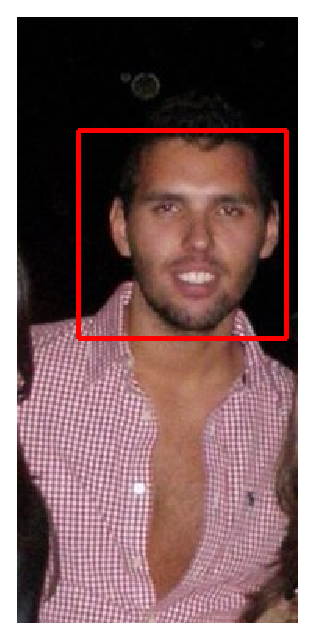
\includegraphics[scale=0.4]{samephoto}
    \caption{ Seleção da face na foto fornecida}
  \end{center}
\end{figure}

Após a seleção da face, o usuário aguarda um breve instante, até que o aplicativo faça a comparação e busca, e assim o resultado será mostrado numa janela. Optamos por mostrar as 6 pessoas com rostos mais parecidos ao rosto alvo, enviado pelo usuário (ver figura 2).

O usuário, então,  escolhe qual dos perfis mostrados é a pessoa que está procurando. No caso em que o perfil é corretamente identificado, o usuário pode simplesmente clicar sobre a foto desejada e ele será redirecionado para a página do perfil dessa pessoa.

No caso de fracasso da busca, o usuário não encontrará o perfil correto entre os 6 mais parecidos, seja porque a pessoa não possui um perfil ou porque o algoritmo não conseguiu encontrar uma foto semelhante. Neste caso, basta fechar a janela.

\begin{center}
  \begin{figure}[h!]
    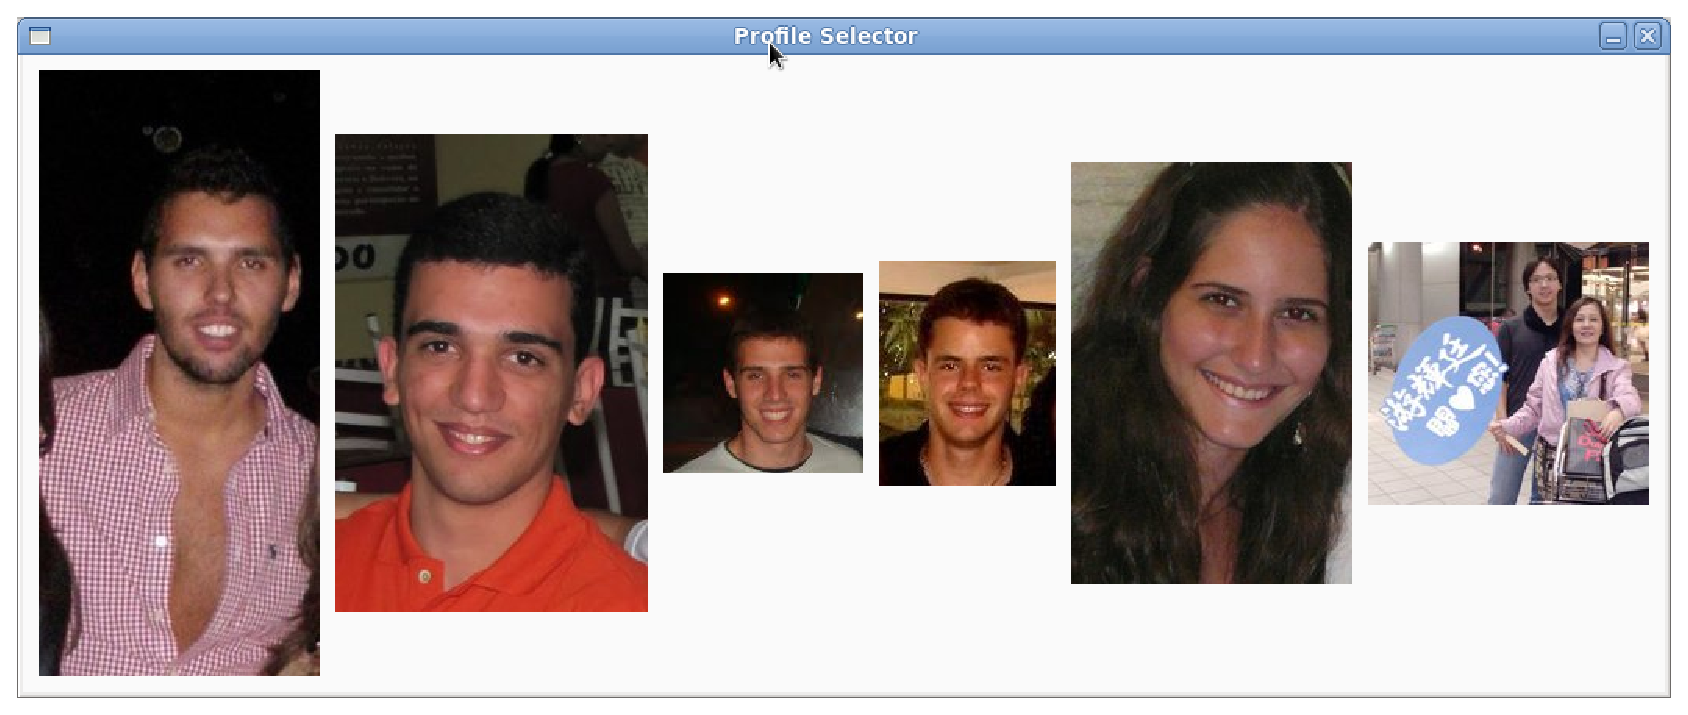
\includegraphics[scale=0.5]{6maisproximos}
    \caption{Faces mais próximas}
  \end{figure}
\end{center}

\section{Exprerimentos}
Ao longo do desenvolvimento do projeto, fizemos algumas medições para encontrarmos
rapidamente qual seriam os possíveis gargalos do aplicativo. E
encontramos problemas na definição do número de usuários que seriam
utilizados na busca, no ajuste da ferramenta que realiza detecção de
faces e no próprio algoritmo do PCA.

\subsubsection*{Definição de espaço}

Como descrito, a primeira abordagem que adotamos foi definir o espaço
que iríamos fazer as buscas. Para isto, implementamos o algoritmo e
executamos algumas vezes.

A primeira versão baixava fotos de perfis do Facebook
sequencialmente, o que casou um certo espanto, pois o tempo
gasto para baixar 2000 fotos era de aproximadamente 70
minutos. Completamente inviável para a nossa proposta de
realizar a busca completa em tempo hábil.

Obviamente, precisávamos fazer este processo em paralelo. E
assim, utilizando threads e requisições em lote, o tempo
baixou de 70 minutos para 1 minuto e meio, também para 2000
fotos. De modo que utilizando o usuário médio, com 130 amigos,
seria razoável realizar a busca apenas entre os amigos de seus
amigos, o que nos daria aproximadamente 17000 pessoas. Ou
seja, por volta de 13 minutos para obter as fotos.

Para esta etapa, parecia razoável, mas este tempo se mostrou ainda
menor no decorrer da implementação.

\subsubsection*{Detecção de faces}

Com as fotos já em disco, precisávamos filtrá-las de forma a
retirar elementos que interferissem mais do que desejaríamos
no resultado da busca. Ou seja, recortar e guardar apenas os
rostos, caso tivessem.

Optamos por utilizar o detector de faces disponível na
biblioteca do OpenCV, mas não para C++, que é mais comum, e sim para python.

Nesta etapa, o foco mudou do tempo gasto para qualidade do
resultado. Pois no caso da definição de espaço, estávamos
interessados em diminuir o intervalo de tempo necessário para
baixar fotos, e na detecção de faces estamos preocupados com a
qualidade das fotos resultantes. Isto é, precisamos encontrar
o maior número de faces, mas não queremos encontrar imagens que não sejam faces.

Conseguimos um bom resultado neste processo. Aproximadamente,
das 2000 fotos que continuamos usando para teste, eram
encontrados em torno de 1350 fotos, ou seja, um aproveitamento
de 67,5\%.

Porém, um outro dado interessante é quantas imagens tinham
realmente rostos. E nas 1350 que o aplicativo dizia ter um
rosto, em torno de 20 não era verdade. Novamente, isto nos dá
um acerto em torno de 85\%.

Considerando os dois resultados, nosso aplicativo obteve uma
taxa de 57\% de acerto ao detectar e recortar rostos. O que
nos pareceu muito bom, pois não conseguimos controlar as fotos
dos usuários, de modo que ele sempre tenha uma foto boa e de face.

\section{Conclusões}

Apesar dos problemas encontrados, a solução proposta utilizando PCA
atende razoavelmente as expectativas. O algoritmo tem performance
excelente quando a foto do perfil é exatamente a buscada, mas possui
um resultado apenas razoável quando elas diferem.

O aplicativo fica exposto a certas limitações que são
inerentes ao problema. Para citar, há casos básicos como a
pessoa não possuir perfil; casos em que não conseguimos
encontrar um rosto na foto de perfil; e casos que mesmo
fazendo a busca por fotos de perfil atuais ou antigas e fotos
marcadas, o algoritmo não consegue encontrar semelhanças entre
duas imagens com a mesma face. Neste caso, geralmente as fotos
possuem características incomuns, tais como rostos virados
para lados opostos, iluminação ou contraste diferentes, 
entre outros elementos.
% ******************************************************
% REFERENCIAS BIBLIOGRÁFICAS
% ******************************************************
% \section{Referências}
\bibliographystyle{plain}
\begin{small}
  \bibliography{referencias}
\end{small}


\end{document}